% Review 2 presentation.
% Build: python scripts/make_tables.py ; cd slides && latexmk -pdf review2.tex
\documentclass[aspectratio=169,10pt]{beamer}
\usetheme[progressbar=frametitle,numbering=fraction,block=fill]{metropolis}
\usepackage[T1]{fontenc}
\usepackage[scaled=0.95]{helvet}
\renewcommand{\familydefault}{\sfdefault}
\usepackage{booktabs}
\usepackage{adjustbox}
\usepackage{tikz}
\usetikzlibrary{arrows.meta,positioning,calc,fit}
\graphicspath{{../results/}}
% generated by scripts/make_tables.py from results/*.csv -- do not edit
\makeatletter
\newcommand\V[1]{\@ifundefined{qv@#1}{\textbf{??#1??}}{\csname qv@#1\endcsname}}
\expandafter\def\csname qv@attacks-rejected\endcsname{21}
\expandafter\def\csname qv@attacks-total\endcsname{21}
\expandafter\def\csname qv@burst-cpu-ags\endcsname{23.3}
\expandafter\def\csname qv@burst-cpu-more\endcsname{65}
\expandafter\def\csname qv@burst-cpu-pbft\endcsname{14.1}
\expandafter\def\csname qv@classic-beacon-aead\endcsname{0.40}
\expandafter\def\csname qv@classic-beacon-aead-bytes\endcsname{135}
\expandafter\def\csname qv@classic-beacon-signed\endcsname{0.88}
\expandafter\def\csname qv@classic-beacon-signed-bytes\endcsname{234}
\expandafter\def\csname qv@classic-beacon-signed-frames\endcsname{1}
\expandafter\def\csname qv@classic-cache-saving\endcsname{34}
\expandafter\def\csname qv@classic-cached-bytes\endcsname{691}
\expandafter\def\csname qv@classic-cached-frames\endcsname{4}
\expandafter\def\csname qv@classic-cached-kb\endcsname{0.7}
\expandafter\def\csname qv@classic-cert\endcsname{229}
\expandafter\def\csname qv@classic-ch\endcsname{323}
\expandafter\def\csname qv@classic-ch-cached\endcsname{165}
\expandafter\def\csname qv@classic-ck\endcsname{216}
\expandafter\def\csname qv@classic-fs\endcsname{70}
\expandafter\def\csname qv@classic-hs-air\endcsname{2.05}
\expandafter\def\csname qv@classic-hs-bytes\endcsname{1{,}043}
\expandafter\def\csname qv@classic-hs-frames\endcsname{4}
\expandafter\def\csname qv@classic-hs-kb\endcsname{1.0}
\expandafter\def\csname qv@classic-hs-ms\endcsname{1.16}
\expandafter\def\csname qv@classic-sh\endcsname{434}
\expandafter\def\csname qv@classic-sh-cached\endcsname{239}
\expandafter\def\csname qv@classic-sig\endcsname{70}
\expandafter\def\csname qv@classic-sign\endcsname{0.031}
\expandafter\def\csname qv@cons-byte-hi\endcsname{30}
\expandafter\def\csname qv@cons-byte-lo\endcsname{8}
\expandafter\def\csname qv@cons-cpu-hi\endcsname{25}
\expandafter\def\csname qv@cons-cpu-lo\endcsname{18}
\expandafter\def\csname qv@cons-lat-hi\endcsname{58}
\expandafter\def\csname qv@cons-lat-lo\endcsname{41}
\expandafter\def\csname qv@cons-msg-8\endcsname{73}
\expandafter\def\csname qv@cons-msg-hi\endcsname{86}
\expandafter\def\csname qv@cons-msg-lo\endcsname{73}
\expandafter\def\csname qv@cons-msg-rest-lo\endcsname{81}
\expandafter\def\csname qv@cons-noshadow-byte-hi\endcsname{64}
\expandafter\def\csname qv@cons-noshadow-byte-lo\endcsname{41}
\expandafter\def\csname qv@deck-beacon-aead\endcsname{0.41}
\expandafter\def\csname qv@deck-beacon-aead-bytes\endcsname{135}
\expandafter\def\csname qv@deck-beacon-signed\endcsname{9.51}
\expandafter\def\csname qv@deck-beacon-signed-bytes\endcsname{3{,}472}
\expandafter\def\csname qv@deck-beacon-signed-frames\endcsname{3}
\expandafter\def\csname qv@deck-beacon-signed-pure\endcsname{236}
\expandafter\def\csname qv@deck-cache-saving\endcsname{51}
\expandafter\def\csname qv@deck-cached-bytes\endcsname{10{,}173}
\expandafter\def\csname qv@deck-cached-frames\endcsname{10}
\expandafter\def\csname qv@deck-cached-kb\endcsname{10.2}
\expandafter\def\csname qv@deck-cert\endcsname{5{,}355}
\expandafter\def\csname qv@deck-ch\endcsname{5{,}446}
\expandafter\def\csname qv@deck-ch-cached\endcsname{162}
\expandafter\def\csname qv@deck-ck\endcsname{4{,}960}
\expandafter\def\csname qv@deck-decaps-native\endcsname{0.052}
\expandafter\def\csname qv@deck-encaps-native\endcsname{0.067}
\expandafter\def\csname qv@deck-fs\endcsname{70}
\expandafter\def\csname qv@deck-hs-air\endcsname{30.5}
\expandafter\def\csname qv@deck-hs-bytes\endcsname{20{,}779}
\expandafter\def\csname qv@deck-hs-frames\endcsname{17}
\expandafter\def\csname qv@deck-hs-kb\endcsname{20.8}
\expandafter\def\csname qv@deck-hs-ms\endcsname{4.77}
\expandafter\def\csname qv@deck-hs-ms-pure\endcsname{209}
\expandafter\def\csname qv@deck-sh\endcsname{10{,}303}
\expandafter\def\csname qv@deck-sh-cached\endcsname{4{,}981}
\expandafter\def\csname qv@deck-sig\endcsname{3{,}309}
\expandafter\def\csname qv@deck-sign-native\endcsname{1.28}
\expandafter\def\csname qv@deck-sign-native-p99\endcsname{4.38}
\expandafter\def\csname qv@deck-sign-pure\endcsname{74.0}
\expandafter\def\csname qv@deck-sign-pure-p99\endcsname{258}
\expandafter\def\csname qv@deck-verify-native\endcsname{0.23}
\expandafter\def\csname qv@l1-beacon-aead\endcsname{0.44}
\expandafter\def\csname qv@l1-beacon-aead-bytes\endcsname{135}
\expandafter\def\csname qv@l1-beacon-signed\endcsname{5.55}
\expandafter\def\csname qv@l1-beacon-signed-bytes\endcsname{2{,}583}
\expandafter\def\csname qv@l1-beacon-signed-frames\endcsname{2}
\expandafter\def\csname qv@l1-beacon-signed-pure\endcsname{105}
\expandafter\def\csname qv@l1-cache-saving\endcsname{53}
\expandafter\def\csname qv@l1-cached-bytes\endcsname{6{,}825}
\expandafter\def\csname qv@l1-cached-frames\endcsname{8}
\expandafter\def\csname qv@l1-cached-kb\endcsname{6.8}
\expandafter\def\csname qv@l1-cert\endcsname{3{,}826}
\expandafter\def\csname qv@l1-ch\endcsname{3{,}915}
\expandafter\def\csname qv@l1-ch-cached\endcsname{160}
\expandafter\def\csname qv@l1-ck\endcsname{3{,}271}
\expandafter\def\csname qv@l1-fs\endcsname{70}
\expandafter\def\csname qv@l1-hs-air\endcsname{21.3}
\expandafter\def\csname qv@l1-hs-bytes\endcsname{14{,}373}
\expandafter\def\csname qv@l1-hs-frames\endcsname{13}
\expandafter\def\csname qv@l1-hs-kb\endcsname{14.4}
\expandafter\def\csname qv@l1-hs-ms\endcsname{11.6}
\expandafter\def\csname qv@l1-hs-ms-pure\endcsname{106}
\expandafter\def\csname qv@l1-sh\endcsname{7{,}117}
\expandafter\def\csname qv@l1-sh-cached\endcsname{3{,}324}
\expandafter\def\csname qv@l1-sig\endcsname{2{,}420}
\expandafter\def\csname qv@l3-beacon-aead\endcsname{0.41}
\expandafter\def\csname qv@l3-beacon-aead-bytes\endcsname{135}
\expandafter\def\csname qv@l3-beacon-signed\endcsname{9.87}
\expandafter\def\csname qv@l3-beacon-signed-bytes\endcsname{3{,}472}
\expandafter\def\csname qv@l3-beacon-signed-frames\endcsname{3}
\expandafter\def\csname qv@l3-beacon-signed-pure\endcsname{194}
\expandafter\def\csname qv@l3-cache-saving\endcsname{53}
\expandafter\def\csname qv@l3-cached-bytes\endcsname{9{,}307}
\expandafter\def\csname qv@l3-cached-frames\endcsname{10}
\expandafter\def\csname qv@l3-cached-kb\endcsname{9.3}
\expandafter\def\csname qv@l3-cert\endcsname{5{,}355}
\expandafter\def\csname qv@l3-ch\endcsname{5{,}444}
\expandafter\def\csname qv@l3-ch-cached\endcsname{160}
\expandafter\def\csname qv@l3-ck\endcsname{4{,}480}
\expandafter\def\csname qv@l3-fs\endcsname{70}
\expandafter\def\csname qv@l3-hs-air\endcsname{29.4}
\expandafter\def\csname qv@l3-hs-bytes\endcsname{19{,}913}
\expandafter\def\csname qv@l3-hs-frames\endcsname{17}
\expandafter\def\csname qv@l3-hs-kb\endcsname{19.9}
\expandafter\def\csname qv@l3-hs-ms\endcsname{4.77}
\expandafter\def\csname qv@l3-hs-ms-pure\endcsname{178}
\expandafter\def\csname qv@l3-sh\endcsname{9{,}919}
\expandafter\def\csname qv@l3-sh-cached\endcsname{4{,}597}
\expandafter\def\csname qv@l3-sig\endcsname{3{,}309}
\expandafter\def\csname qv@l5-beacon-aead\endcsname{0.47}
\expandafter\def\csname qv@l5-beacon-aead-bytes\endcsname{135}
\expandafter\def\csname qv@l5-beacon-signed\endcsname{12.6}
\expandafter\def\csname qv@l5-beacon-signed-bytes\endcsname{4{,}790}
\expandafter\def\csname qv@l5-beacon-signed-frames\endcsname{4}
\expandafter\def\csname qv@l5-beacon-signed-pure\endcsname{184}
\expandafter\def\csname qv@l5-cache-saving\endcsname{53}
\expandafter\def\csname qv@l5-cached-bytes\endcsname{12{,}807}
\expandafter\def\csname qv@l5-cached-frames\endcsname{12}
\expandafter\def\csname qv@l5-cached-kb\endcsname{12.8}
\expandafter\def\csname qv@l5-cert\endcsname{7{,}313}
\expandafter\def\csname qv@l5-ch\endcsname{7{,}402}
\expandafter\def\csname qv@l5-ch-cached\endcsname{160}
\expandafter\def\csname qv@l5-ck\endcsname{6{,}278}
\expandafter\def\csname qv@l5-fs\endcsname{70}
\expandafter\def\csname qv@l5-hs-air\endcsname{40.1}
\expandafter\def\csname qv@l5-hs-bytes\endcsname{27{,}329}
\expandafter\def\csname qv@l5-hs-frames\endcsname{22}
\expandafter\def\csname qv@l5-hs-kb\endcsname{27.3}
\expandafter\def\csname qv@l5-hs-ms\endcsname{5.68}
\expandafter\def\csname qv@l5-hs-ms-pure\endcsname{219}
\expandafter\def\csname qv@l5-sh\endcsname{13{,}579}
\expandafter\def\csname qv@l5-sh-cached\endcsname{6{,}299}
\expandafter\def\csname qv@l5-sig\endcsname{4{,}627}
\expandafter\def\csname qv@net-alert-ms\endcsname{5.4}
\expandafter\def\csname qv@net-beacons\endcsname{11{,}089}
\expandafter\def\csname qv@net-commit-ms\endcsname{51}
\expandafter\def\csname qv@net-handshakes\endcsname{48}
\expandafter\def\csname qv@net-hs-max\endcsname{20{,}779}
\expandafter\def\csname qv@net-hs-min\endcsname{10{,}173}
\expandafter\def\csname qv@net-ledger-ms\endcsname{62}
\expandafter\def\csname qv@net-rejected\endcsname{6}
\expandafter\def\csname qv@net-v2v-ms\endcsname{1.0}
\expandafter\def\csname qv@ns3-airtime-classic-100\endcsname{41}
\expandafter\def\csname qv@ns3-airtime-classic-150\endcsname{61}
\expandafter\def\csname qv@ns3-airtime-classic-200\endcsname{81}
\expandafter\def\csname qv@ns3-airtime-classic-50\endcsname{22}
\expandafter\def\csname qv@ns3-airtime-deck-100\endcsname{160}
\expandafter\def\csname qv@ns3-airtime-deck-150\endcsname{268}
\expandafter\def\csname qv@ns3-airtime-deck-200\endcsname{303}
\expandafter\def\csname qv@ns3-airtime-deck-50\endcsname{40}
\expandafter\def\csname qv@ns3-airtime-deck-cache-100\endcsname{68}
\expandafter\def\csname qv@ns3-airtime-deck-cache-150\endcsname{174}
\expandafter\def\csname qv@ns3-airtime-deck-cache-200\endcsname{258}
\expandafter\def\csname qv@ns3-airtime-deck-cache-50\endcsname{31}
\expandafter\def\csname qv@ns3-airtime-l1-100\endcsname{81}
\expandafter\def\csname qv@ns3-airtime-l1-150\endcsname{246}
\expandafter\def\csname qv@ns3-airtime-l1-200\endcsname{283}
\expandafter\def\csname qv@ns3-airtime-l1-50\endcsname{36}
\expandafter\def\csname qv@ns3-airtime-l3-100\endcsname{175}
\expandafter\def\csname qv@ns3-airtime-l3-150\endcsname{263}
\expandafter\def\csname qv@ns3-airtime-l3-200\endcsname{301}
\expandafter\def\csname qv@ns3-airtime-l3-50\endcsname{38}
\expandafter\def\csname qv@ns3-airtime-l5-100\endcsname{218}
\expandafter\def\csname qv@ns3-airtime-l5-150\endcsname{282}
\expandafter\def\csname qv@ns3-airtime-l5-200\endcsname{318}
\expandafter\def\csname qv@ns3-airtime-l5-50\endcsname{61}
\expandafter\def\csname qv@ns3-airtimepct-classic-100\endcsname{41}
\expandafter\def\csname qv@ns3-airtimepct-deck-100\endcsname{160}
\expandafter\def\csname qv@ns3-airtimepct-deck-cache-100\endcsname{68}
\expandafter\def\csname qv@ns3-alert-classic-100\endcsname{5.4}
\expandafter\def\csname qv@ns3-alert-classic-150\endcsname{5.5}
\expandafter\def\csname qv@ns3-alert-classic-200\endcsname{5.7}
\expandafter\def\csname qv@ns3-alert-classic-50\endcsname{5.2}
\expandafter\def\csname qv@ns3-alert-deck-100\endcsname{7.6}
\expandafter\def\csname qv@ns3-alert-deck-150\endcsname{105.7}
\expandafter\def\csname qv@ns3-alert-deck-200\endcsname{218.4}
\expandafter\def\csname qv@ns3-alert-deck-50\endcsname{5.6}
\expandafter\def\csname qv@ns3-alert-deck-cache-100\endcsname{5.6}
\expandafter\def\csname qv@ns3-alert-deck-cache-150\endcsname{7.7}
\expandafter\def\csname qv@ns3-alert-deck-cache-200\endcsname{33.0}
\expandafter\def\csname qv@ns3-alert-deck-cache-50\endcsname{5.5}
\expandafter\def\csname qv@ns3-alert-l1-100\endcsname{5.6}
\expandafter\def\csname qv@ns3-alert-l1-150\endcsname{70.5}
\expandafter\def\csname qv@ns3-alert-l1-200\endcsname{191.1}
\expandafter\def\csname qv@ns3-alert-l1-50\endcsname{5.4}
\expandafter\def\csname qv@ns3-alert-l3-100\endcsname{11.4}
\expandafter\def\csname qv@ns3-alert-l3-150\endcsname{93.4}
\expandafter\def\csname qv@ns3-alert-l3-200\endcsname{191.6}
\expandafter\def\csname qv@ns3-alert-l3-50\endcsname{5.5}
\expandafter\def\csname qv@ns3-alert-l5-100\endcsname{16.5}
\expandafter\def\csname qv@ns3-alert-l5-150\endcsname{126.7}
\expandafter\def\csname qv@ns3-alert-l5-200\endcsname{273.0}
\expandafter\def\csname qv@ns3-alert-l5-50\endcsname{5.6}
\expandafter\def\csname qv@ns3-alertp50ms-classic-100\endcsname{5.4}
\expandafter\def\csname qv@ns3-alertp50ms-deck-100\endcsname{7.6}
\expandafter\def\csname qv@ns3-alertp50ms-deck-cache-100\endcsname{5.6}
\expandafter\def\csname qv@ns3-beaconcoveragepct-classic-100\endcsname{99.9}
\expandafter\def\csname qv@ns3-beaconcoveragepct-deck-100\endcsname{83.3}
\expandafter\def\csname qv@ns3-beaconcoveragepct-deck-cache-100\endcsname{97.4}
\expandafter\def\csname qv@ns3-commitp50ms-classic-100\endcsname{11.6}
\expandafter\def\csname qv@ns3-commitp50ms-deck-100\endcsname{24.6}
\expandafter\def\csname qv@ns3-commitp50ms-deck-cache-100\endcsname{24.0}
\expandafter\def\csname qv@ns3-coverage-classic-100\endcsname{99.9}
\expandafter\def\csname qv@ns3-coverage-classic-150\endcsname{99.9}
\expandafter\def\csname qv@ns3-coverage-classic-200\endcsname{99.9}
\expandafter\def\csname qv@ns3-coverage-classic-50\endcsname{99.7}
\expandafter\def\csname qv@ns3-coverage-deck-100\endcsname{83.3}
\expandafter\def\csname qv@ns3-coverage-deck-150\endcsname{52.7}
\expandafter\def\csname qv@ns3-coverage-deck-200\endcsname{38.7}
\expandafter\def\csname qv@ns3-coverage-deck-50\endcsname{99.0}
\expandafter\def\csname qv@ns3-coverage-deck-cache-100\endcsname{97.4}
\expandafter\def\csname qv@ns3-coverage-deck-cache-150\endcsname{83.0}
\expandafter\def\csname qv@ns3-coverage-deck-cache-200\endcsname{62.4}
\expandafter\def\csname qv@ns3-coverage-deck-cache-50\endcsname{99.6}
\expandafter\def\csname qv@ns3-coverage-l1-100\endcsname{95.9}
\expandafter\def\csname qv@ns3-coverage-l1-150\endcsname{66.6}
\expandafter\def\csname qv@ns3-coverage-l1-200\endcsname{52.5}
\expandafter\def\csname qv@ns3-coverage-l1-50\endcsname{99.4}
\expandafter\def\csname qv@ns3-coverage-l3-100\endcsname{78.1}
\expandafter\def\csname qv@ns3-coverage-l3-150\endcsname{51.9}
\expandafter\def\csname qv@ns3-coverage-l3-200\endcsname{37.4}
\expandafter\def\csname qv@ns3-coverage-l3-50\endcsname{99.0}
\expandafter\def\csname qv@ns3-coverage-l5-100\endcsname{67.5}
\expandafter\def\csname qv@ns3-coverage-l5-150\endcsname{44.4}
\expandafter\def\csname qv@ns3-coverage-l5-200\endcsname{31.3}
\expandafter\def\csname qv@ns3-coverage-l5-50\endcsname{96.4}
\expandafter\def\csname qv@ns3-hsp95ms-classic-100\endcsname{33}
\expandafter\def\csname qv@ns3-hsp95ms-deck-100\endcsname{1{,}094}
\expandafter\def\csname qv@ns3-hsp95ms-deck-cache-100\endcsname{359}
\expandafter\def\csname qv@ns3-linkslost-classic-100\endcsname{0.0}
\expandafter\def\csname qv@ns3-linkslost-deck-100\endcsname{3.0}
\expandafter\def\csname qv@ns3-linkslost-deck-cache-100\endcsname{1.7}
\expandafter\def\csname qv@ns3-mid\endcsname{100}
\expandafter\def\csname qv@ns3-p50-classic-100\endcsname{8}
\expandafter\def\csname qv@ns3-p50-classic-150\endcsname{10}
\expandafter\def\csname qv@ns3-p50-classic-200\endcsname{12}
\expandafter\def\csname qv@ns3-p50-classic-50\endcsname{7}
\expandafter\def\csname qv@ns3-p50-deck-100\endcsname{285}
\expandafter\def\csname qv@ns3-p50-deck-150\endcsname{636}
\expandafter\def\csname qv@ns3-p50-deck-200\endcsname{795}
\expandafter\def\csname qv@ns3-p50-deck-50\endcsname{90}
\expandafter\def\csname qv@ns3-p50-deck-cache-100\endcsname{73}
\expandafter\def\csname qv@ns3-p50-deck-cache-150\endcsname{197}
\expandafter\def\csname qv@ns3-p50-deck-cache-200\endcsname{417}
\expandafter\def\csname qv@ns3-p50-deck-cache-50\endcsname{54}
\expandafter\def\csname qv@ns3-p50-l1-100\endcsname{109}
\expandafter\def\csname qv@ns3-p50-l1-150\endcsname{575}
\expandafter\def\csname qv@ns3-p50-l1-200\endcsname{763}
\expandafter\def\csname qv@ns3-p50-l1-50\endcsname{73}
\expandafter\def\csname qv@ns3-p50-l3-100\endcsname{288}
\expandafter\def\csname qv@ns3-p50-l3-150\endcsname{651}
\expandafter\def\csname qv@ns3-p50-l3-200\endcsname{760}
\expandafter\def\csname qv@ns3-p50-l3-50\endcsname{88}
\expandafter\def\csname qv@ns3-p50-l5-100\endcsname{482}
\expandafter\def\csname qv@ns3-p50-l5-150\endcsname{750}
\expandafter\def\csname qv@ns3-p50-l5-200\endcsname{844}
\expandafter\def\csname qv@ns3-p50-l5-50\endcsname{139}
\expandafter\def\csname qv@ns3-p95-classic-100\endcsname{33}
\expandafter\def\csname qv@ns3-p95-classic-150\endcsname{48}
\expandafter\def\csname qv@ns3-p95-classic-200\endcsname{51}
\expandafter\def\csname qv@ns3-p95-classic-50\endcsname{27}
\expandafter\def\csname qv@ns3-p95-deck-100\endcsname{1{,}094}
\expandafter\def\csname qv@ns3-p95-deck-150\endcsname{1{,}265}
\expandafter\def\csname qv@ns3-p95-deck-200\endcsname{1{,}274}
\expandafter\def\csname qv@ns3-p95-deck-50\endcsname{266}
\expandafter\def\csname qv@ns3-p95-deck-cache-100\endcsname{359}
\expandafter\def\csname qv@ns3-p95-deck-cache-150\endcsname{1{,}057}
\expandafter\def\csname qv@ns3-p95-deck-cache-200\endcsname{1{,}214}
\expandafter\def\csname qv@ns3-p95-deck-cache-50\endcsname{138}
\expandafter\def\csname qv@ns3-p95-l1-100\endcsname{472}
\expandafter\def\csname qv@ns3-p95-l1-150\endcsname{1{,}217}
\expandafter\def\csname qv@ns3-p95-l1-200\endcsname{1{,}250}
\expandafter\def\csname qv@ns3-p95-l1-50\endcsname{201}
\expandafter\def\csname qv@ns3-p95-l3-100\endcsname{1{,}070}
\expandafter\def\csname qv@ns3-p95-l3-150\endcsname{1{,}244}
\expandafter\def\csname qv@ns3-p95-l3-200\endcsname{1{,}252}
\expandafter\def\csname qv@ns3-p95-l3-50\endcsname{251}
\expandafter\def\csname qv@ns3-p95-l5-100\endcsname{1{,}155}
\expandafter\def\csname qv@ns3-p95-l5-150\endcsname{1{,}302}
\expandafter\def\csname qv@ns3-p95-l5-200\endcsname{1{,}265}
\expandafter\def\csname qv@ns3-p95-l5-50\endcsname{472}
\expandafter\def\csname qv@ns3-seeds\endcsname{3}
\expandafter\def\csname qv@ns3-success-classic-100\endcsname{100}
\expandafter\def\csname qv@ns3-success-classic-150\endcsname{100}
\expandafter\def\csname qv@ns3-success-classic-200\endcsname{100}
\expandafter\def\csname qv@ns3-success-classic-50\endcsname{100}
\expandafter\def\csname qv@ns3-success-deck-100\endcsname{74}
\expandafter\def\csname qv@ns3-success-deck-150\endcsname{38}
\expandafter\def\csname qv@ns3-success-deck-200\endcsname{27}
\expandafter\def\csname qv@ns3-success-deck-50\endcsname{100}
\expandafter\def\csname qv@ns3-success-deck-cache-100\endcsname{98}
\expandafter\def\csname qv@ns3-success-deck-cache-150\endcsname{80}
\expandafter\def\csname qv@ns3-success-deck-cache-200\endcsname{57}
\expandafter\def\csname qv@ns3-success-deck-cache-50\endcsname{100}
\expandafter\def\csname qv@ns3-success-l1-100\endcsname{97}
\expandafter\def\csname qv@ns3-success-l1-150\endcsname{54}
\expandafter\def\csname qv@ns3-success-l1-200\endcsname{39}
\expandafter\def\csname qv@ns3-success-l1-50\endcsname{100}
\expandafter\def\csname qv@ns3-success-l3-100\endcsname{70}
\expandafter\def\csname qv@ns3-success-l3-150\endcsname{40}
\expandafter\def\csname qv@ns3-success-l3-200\endcsname{27}
\expandafter\def\csname qv@ns3-success-l3-50\endcsname{99}
\expandafter\def\csname qv@ns3-success-l5-100\endcsname{56}
\expandafter\def\csname qv@ns3-success-l5-150\endcsname{32}
\expandafter\def\csname qv@ns3-success-l5-200\endcsname{22}
\expandafter\def\csname qv@ns3-success-l5-50\endcsname{99}
\expandafter\def\csname qv@pq-cache-hi\endcsname{53}
\expandafter\def\csname qv@pq-cache-lo\endcsname{51}
\expandafter\def\csname qv@pq-size-ratio-hi\endcsname{26}
\expandafter\def\csname qv@pq-size-ratio-lo\endcsname{14}
\expandafter\def\csname qv@sign-speedup\endcsname{58}
\expandafter\def\csname qv@tps-ags\endcsname{47}
\expandafter\def\csname qv@tps-pbft\endcsname{69}
\expandafter\def\csname qv@var-classical-signed-beacons-alert\endcsname{5.4}
\expandafter\def\csname qv@var-classical-signed-beacons-coverage\endcsname{100}
\expandafter\def\csname qv@var-classical-signed-beacons-p50\endcsname{9}
\expandafter\def\csname qv@var-classical-signed-beacons-success\endcsname{100}
\expandafter\def\csname qv@var-deck-backoff-only-alert\endcsname{8.9}
\expandafter\def\csname qv@var-deck-backoff-only-coverage\endcsname{85}
\expandafter\def\csname qv@var-deck-backoff-only-p50\endcsname{291}
\expandafter\def\csname qv@var-deck-backoff-only-success\endcsname{77}
\expandafter\def\csname qv@var-deck-cache-all-warm-alert\endcsname{6.0}
\expandafter\def\csname qv@var-deck-cache-all-warm-coverage\endcsname{99}
\expandafter\def\csname qv@var-deck-cache-all-warm-p50\endcsname{66}
\expandafter\def\csname qv@var-deck-cache-all-warm-success\endcsname{97}
\expandafter\def\csname qv@var-deck-cache-directory-alert\endcsname{5.5}
\expandafter\def\csname qv@var-deck-cache-directory-coverage\endcsname{98}
\expandafter\def\csname qv@var-deck-cache-directory-p50\endcsname{68}
\expandafter\def\csname qv@var-deck-cache-directory-success\endcsname{100}
\expandafter\def\csname qv@var-deck-edca-backoff-baseline-alert\endcsname{7.2}
\expandafter\def\csname qv@var-deck-edca-backoff-baseline-coverage\endcsname{82}
\expandafter\def\csname qv@var-deck-edca-backoff-baseline-p50\endcsname{283}
\expandafter\def\csname qv@var-deck-edca-backoff-baseline-success\endcsname{75}
\expandafter\def\csname qv@var-deck-edca-only-alert\endcsname{382.3}
\expandafter\def\csname qv@var-deck-edca-only-coverage\endcsname{44}
\expandafter\def\csname qv@var-deck-edca-only-p50\endcsname{926}
\expandafter\def\csname qv@var-deck-edca-only-success\endcsname{11}
\expandafter\def\csname qv@var-deck-neither-alert\endcsname{432.6}
\expandafter\def\csname qv@var-deck-neither-coverage\endcsname{40}
\expandafter\def\csname qv@var-deck-neither-p50\endcsname{921}
\expandafter\def\csname qv@var-deck-neither-success\endcsname{7}
\expandafter\def\csname qv@var-deck-pure-python-timings-alert\endcsname{8.6}
\expandafter\def\csname qv@var-deck-pure-python-timings-coverage\endcsname{74}
\expandafter\def\csname qv@var-deck-pure-python-timings-p50\endcsname{593}
\expandafter\def\csname qv@var-deck-pure-python-timings-success\endcsname{69}
\expandafter\def\csname qv@var-deck-signed-beacons-alert\endcsname{232.9}
\expandafter\def\csname qv@var-deck-signed-beacons-coverage\endcsname{46}
\expandafter\def\csname qv@var-deck-signed-beacons-p50\endcsname{704}
\expandafter\def\csname qv@var-deck-signed-beacons-success\endcsname{23}
\expandafter\def\csname qv@var-l3-cache-directory-alert\endcsname{5.9}
\expandafter\def\csname qv@var-l3-cache-directory-coverage\endcsname{97}
\expandafter\def\csname qv@var-l3-cache-directory-p50\endcsname{76}
\expandafter\def\csname qv@var-l3-cache-directory-success\endcsname{100}
\makeatother


\definecolor{ink}{HTML}{1B211F}
\definecolor{teal}{HTML}{0F7A63}
\definecolor{amber}{HTML}{C27100}
\definecolor{brick}{HTML}{C0392B}
\definecolor{paper}{HTML}{F7F8F5}
\setbeamercolor{normal text}{fg=ink,bg=paper}
\setbeamercolor{frametitle}{bg=ink,fg=paper}
\setbeamercolor{progress bar}{fg=teal,bg=ink!20}
\setbeamercolor{alerted text}{fg=brick}
\setbeamercolor{example text}{fg=teal}
\setbeamercolor{title separator}{fg=teal}
\newcommand{\bignum}[1]{{\Large\bfseries #1}}
\newcommand{\code}[1]{\texttt{#1}}

\title{Quantum-Resilient Authenticated Communication\\for Connected Autonomous Vehicles}
\subtitle{Review 2: the complete system and its evaluation}
\author{Harini R \quad Ananyalakshmi V K \quad Adhithya K \quad Ratish S A\\[2pt]
\small Guide: Dr.\ Vijayalakshmi M}
\institute{Department of Information Technology, College of Engineering Guindy, Anna University}
\date{}

\begin{document}

\maketitle

% -----------------------------------------------------------------------------
\begin{frame}{The problem}
\begin{columns}[T]
\begin{column}{0.55\textwidth}
\begin{itemize}
\item V2X safety messages are signed with \textbf{ECDSA} and keyed with \textbf{ECDH} (IEEE 1609.2).
\item \textbf{Shor's algorithm breaks both.} Traffic recorded today can be decrypted later.
\item Cars stay on the road 15+ years: a car sold now must be secure in 2040.
\item NIST standardised the replacements in 2024: \textbf{ML-KEM} (FIPS 203) and \textbf{ML-DSA} (FIPS 204).
\end{itemize}
\end{column}
\begin{column}{0.42\textwidth}
\begin{block}{The catch: size}
\small
\begin{tabular}{@{}lrr@{}}
& ECDSA P-256 & ML-DSA-65 \\
\midrule
public key & 65 B & 1,952 B \\
signature & $\approx$70 B & 3,309 B \\
certificate & \V{classic-cert} B & \V{deck-cert} B \\
\end{tabular}
\end{block}
\vspace{4pt}
\small 802.11p: 6\,Mb/s, shared by every vehicle in range, beacons every 100\,ms.
\end{column}
\end{columns}
\end{frame}

% -----------------------------------------------------------------------------
\begin{frame}{What we set out to do, and where we are}
\begin{columns}[T]
\begin{column}{0.5\textwidth}
\textbf{Objectives}
\begin{enumerate}
\item Implement the base paper's framework end to end with ML-KEM and ML-DSA
\item Fix what prevents it from working
\item Measure compute, size and airtime vs a classical baseline
\item Evaluate on an 802.11p channel with mobility (ns-3)
\item Compare AGS-PBFT with PBFT
\item Attack it
\end{enumerate}
\end{column}
\begin{column}{0.46\textwidth}
\textbf{Status}
\begin{itemize}
\item[\textcolor{teal}{\checkmark}] Distributed system: 19 processes over TCP
\item[\textcolor{teal}{\checkmark}] ns-3: 5 suites + caching $\times$ 50--200 vehicles $\times$ \V{ns3-seeds} seeds
\item[\textcolor{teal}{\checkmark}] \V{attacks-total} attacks, \V{attacks-rejected} rejected
\item[\textcolor{teal}{\checkmark}] 57 automated tests
\item[\textcolor{teal}{\checkmark}] New: certificate caching (handshake $-$\V{deck-cache-saving}\,\%)
\item[\textcolor{teal}{\checkmark}] Replay viewer for the simulation
\end{itemize}
\end{column}
\end{columns}
\end{frame}

% -----------------------------------------------------------------------------
\begin{frame}{Architecture}
\centering
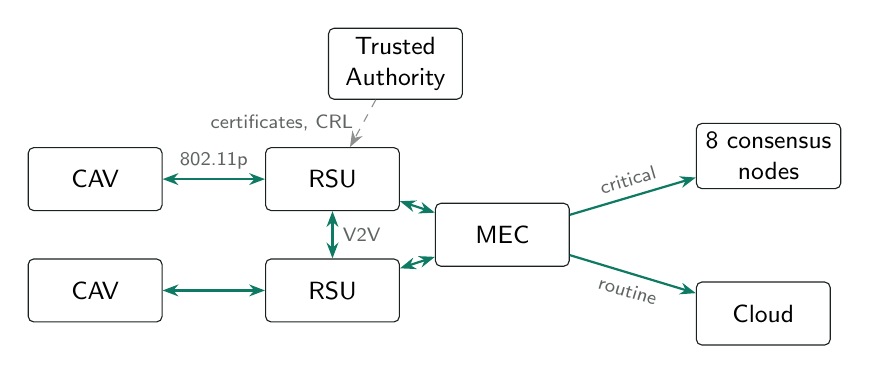
\begin{tikzpicture}[
  node distance=6mm and 9mm,
  box/.style={draw=ink, fill=white, rounded corners=2pt, minimum height=8mm, minimum width=17mm, align=center, font=\small},
  lab/.style={font=\scriptsize, align=center, text=ink!70},
  >={Stealth[length=2mm]}]
\node[box] (cav1) {CAV};
\node[box, below=of cav1] (cav2) {CAV};
\node[box, right=13mm of cav1] (rsu1) {RSU};
\node[box, right=13mm of cav2] (rsu2) {RSU};
\node[box, right=13mm of $(rsu1)!0.5!(rsu2)$] (mec) {MEC};
\node[box, right=16mm of mec, yshift=10mm] (cons) {8 consensus\\nodes};
\node[box, right=16mm of mec, yshift=-10mm] (cloud) {Cloud};
\node[box, above=6mm of rsu1, xshift=8mm] (ta) {Trusted\\Authority};
\draw[<->, teal, thick] (cav1) -- node[lab, above]{802.11p} (rsu1);
\draw[<->, teal, thick] (cav2) -- (rsu2);
\draw[<->, teal, thick] (rsu1) -- node[lab, right]{V2V} (rsu2);
\draw[<->, teal, thick] (rsu1) -- (mec);
\draw[<->, teal, thick] (rsu2) -- (mec);
\draw[->, teal, thick] (mec) -- node[lab, above, sloped]{critical} (cons);
\draw[->, teal, thick] (mec) -- node[lab, below, sloped]{routine} (cloud);
\draw[->, dashed, ink!50] (ta) -- node[lab, left]{certificates, CRL} (rsu1);
\end{tikzpicture}

\vspace{6pt}
\small Every \textcolor{teal}{green} link is a mutually authenticated ML-KEM + ML-DSA session carrying AES-256-GCM records.\\
The MEC sends the \textbf{alert first}, then submits the event to consensus: safety never waits for the ledger.
\end{frame}

% -----------------------------------------------------------------------------
\begin{frame}{The base paper cannot run as written}
\small
\begin{tabular}{@{}p{0.5cm}p{6.6cm}p{6.6cm}@{}}
\toprule
& In the paper & What we do \\
\midrule
D1 & Consensus messages ``signed with Kyber''. \textbf{A KEM cannot sign.} & ML-DSA signatures \\
D2 & Encapsulation defines $k_i$ using $k_i$ & standard Encaps / Decaps \\
D3 & Session key $= H(k_i \parallel k'_j)$ with $k_i = k'_j$ & HKDF over secret + transcript hash \\
D4 & TA generates private keys, yet claims ``no key escrow'' & entities make their own keys; proof of possession \\
D5 & Hyperledger Fabric 2.2 uses Raft: cannot host PBFT & our own certified ledger \\
\bottomrule
\end{tabular}

\vspace{8pt}
And four gaps in AGS-PBFT itself (D6--D9): $\sigma = 0$ at the first regroup, candidates that can never be promoted, undefined group sizing, an unreachable prepare quorum.
\end{frame}

% -----------------------------------------------------------------------------
\begin{frame}{Handshake: four flights, both sides authenticated}
\begin{columns}[T]
\begin{column}{0.56\textwidth}
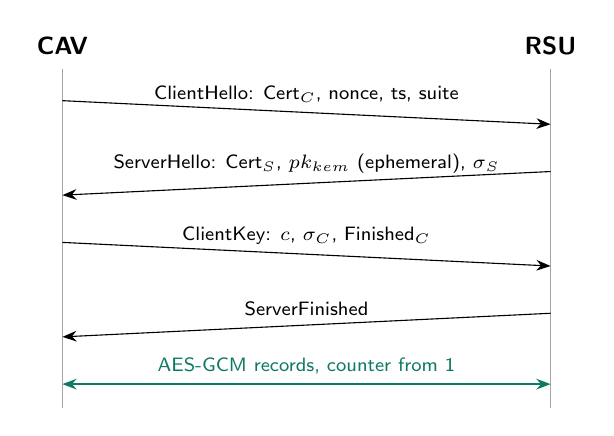
\begin{tikzpicture}[font=\scriptsize, >={Stealth[length=1.8mm]}]
\def\L{0} \def\R{6.2}
\node[font=\small\bfseries] at (\L,0.3) {CAV}; \node[font=\small\bfseries] at (\R,0.3) {RSU};
\draw[ink!40] (\L,0) -- (\L,-4.3); \draw[ink!40] (\R,0) -- (\R,-4.3);
\draw[->] (\L,-0.4) -- node[above]{ClientHello: Cert$_C$, nonce, ts, suite} (\R,-0.7);
\draw[<-] (\L,-1.6) -- node[above]{ServerHello: Cert$_S$, $pk_{kem}$ (ephemeral), $\sigma_S$} (\R,-1.3);
\draw[->] (\L,-2.2) -- node[above]{ClientKey: $c$, $\sigma_C$, Finished$_C$} (\R,-2.5);
\draw[<-] (\L,-3.4) -- node[above]{ServerFinished} (\R,-3.1);
\draw[<->, teal, thick] (\L,-4.0) -- node[above]{AES-GCM records, counter from 1} (\R,-4.0);
\end{tikzpicture}
\end{column}
\begin{column}{0.42\textwidth}
\small
Fixes to our Review 1 design:
\begin{itemize}
\item \textbf{F2: the client now signs.} Before, a copied (public) certificate was enough to impersonate a vehicle.
\item F1: ClientHello nonce opens the transcript.
\item F3: data counter starts at 1: no GCM nonce reuse.
\item F5--F7: role in certificate, downgrade protection, uniform abort.
\end{itemize}
Forward secrecy: the RSU's KEM key is erased after each session.
\end{column}
\end{columns}
\end{frame}

% -----------------------------------------------------------------------------
\begin{frame}{New: certificate caching}
\begin{columns}[T]
\begin{column}{0.5\textwidth}
\small
Half the handshake is two 5.3\,KB certificates. Peers usually hold them already:
\begin{itemize}
\item RSU certificates: \textbf{pre-distributed} with the CRL
\item vehicle certificates: \textbf{edge directory} at the MEC after first contact
\end{itemize}
Send $H(\text{cert})$, 32 bytes, instead. Unknown reference $\rightarrow$ HelloRetry, then the full certificate.

\vspace{4pt}
\textbf{Security:} cached certificates are still verified every time (TA signature, CRL); the reference is inside both signatures; caching only after a completed handshake.
\end{column}
\begin{column}{0.47\textwidth}
\centering
\begin{tabular}{@{}lrr@{}}
\toprule
DECK & full & cached \\
\midrule
ClientHello & \V{deck-ch} & \V{deck-ch-cached} \\
ServerHello & \V{deck-sh} & \V{deck-sh-cached} \\
ClientKey & \V{deck-ck} & \V{deck-ck} \\
ServerFinished & \V{deck-fs} & \V{deck-fs} \\
\midrule
\textbf{total (B)} & \textbf{\V{deck-hs-bytes}} & \textbf{\V{deck-cached-bytes}} \\
radio frames & \V{deck-hs-frames} & \V{deck-cached-frames} \\
\bottomrule
\end{tabular}

\vspace{6pt}
\bignum{$-$\V{deck-cache-saving}\,\%}
\end{column}
\end{columns}
\end{frame}

% -----------------------------------------------------------------------------
\begin{frame}{AGS-PBFT}
\small
\begin{columns}[T]
\begin{column}{0.52\textwidth}
\begin{enumerate}
\item MEC $\rightarrow$ leader: signed REQUEST
\item PRE-PREPARE $\rightarrow$ consensus set (+ candidates)
\item PREPARE all-to-all; each node validates the event
\item RESPONSE $\rightarrow$ leader; $2f+1$ match $\rightarrow$ signed block with commit certificate
\item Every node re-verifies the block, scores and membership
\end{enumerate}
\end{column}
\begin{column}{0.45\textwidth}
\begin{itemize}
\item Score $+1$ agree, $-5$ disagree
\item Every $k$ blocks: demote below $\mu-\sigma$, promote above $\mu+\sigma$
\item View change when the leader is silent
\item PBFT baseline with the same signatures
\end{itemize}
\end{column}
\end{columns}
\end{frame}

% -----------------------------------------------------------------------------
\begin{frame}{Implementation}
\small
\begin{columns}[T]
\begin{column}{0.48\textwidth}
\textbf{Runs three ways}
\begin{enumerate}
\item \textbf{Distributed}: TA, cloud, MEC, 8 nodes, 3 RSUs, 5 vehicles as 19 processes; faults injected (Byzantine node, leader crash, revocation)
\item \textbf{ns-3}: IEEE 802.11p, Nakagami fading, Manhattan mobility, 9 RSUs; real message sizes and measured processing times
\item \textbf{Evaluation suite}: benchmarks, attacks, consensus experiments, figures
\end{enumerate}
\end{column}
\begin{column}{0.48\textwidth}
\textbf{Stack}
\begin{itemize}
\item Python, \code{cryptography} (OpenSSL 3.5: native ML-KEM / ML-DSA)
\item \code{kyber-py}, \code{dilithium-py}: pure-Python comparison backend
\item ns-3 3.44 (C++ scenario via Python bindings)
\item 5 suites: Classical, L1, L3, DECK (1024/65), L5
\item Classical runs through the \textbf{same protocol code}
\end{itemize}
\end{column}
\end{columns}
\end{frame}

% -----------------------------------------------------------------------------
\begin{frame}{Result 1: compute is small, bytes are not}
\begin{columns}[c]
\begin{column}{0.58\textwidth}
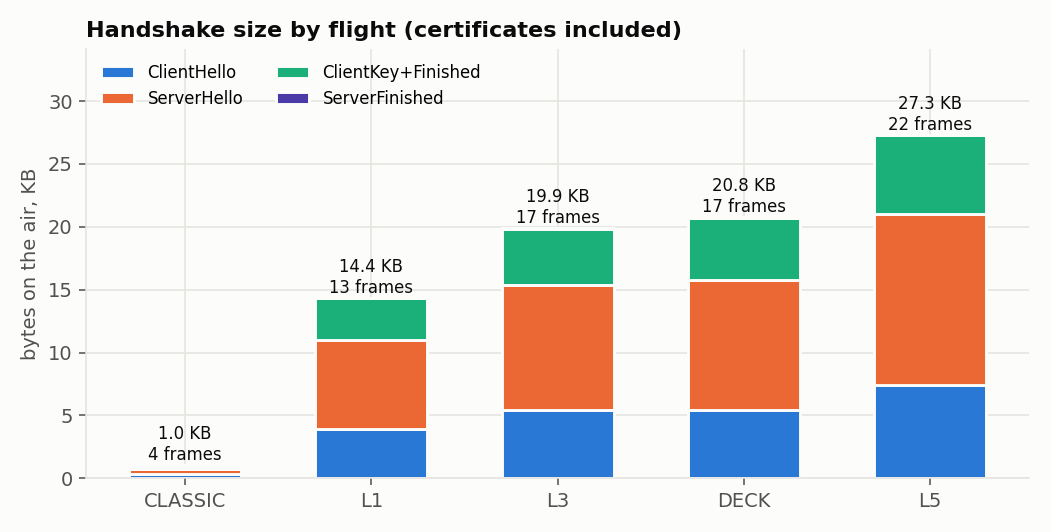
\includegraphics[width=\textwidth]{fig2_handshake_size.png}
\end{column}
\begin{column}{0.4\textwidth}
\small
\begin{tabular}{@{}lrr@{}}
& Classical & DECK \\
\midrule
bytes & \V{classic-hs-bytes} & \V{deck-hs-bytes} \\
frames & \V{classic-hs-frames} & \V{deck-hs-frames} \\
airtime (ms) & \V{classic-hs-air} & \V{deck-hs-air} \\
compute, native (ms) & \V{classic-hs-ms} & \V{deck-hs-ms} \\
compute, pure (ms) & -- & \V{deck-hs-ms-pure} \\
\end{tabular}

\vspace{6pt}
ML-DSA-65 signs in \V{deck-sign-native}\,ms natively vs \V{deck-sign-pure}\,ms in pure Python: \textbf{implementation matters more than the algorithm}.
\end{column}
\end{columns}
\end{frame}

% -----------------------------------------------------------------------------
\begin{frame}{Result 2: per message, post-quantum fits}
\begin{columns}[c]
\begin{column}{0.58\textwidth}
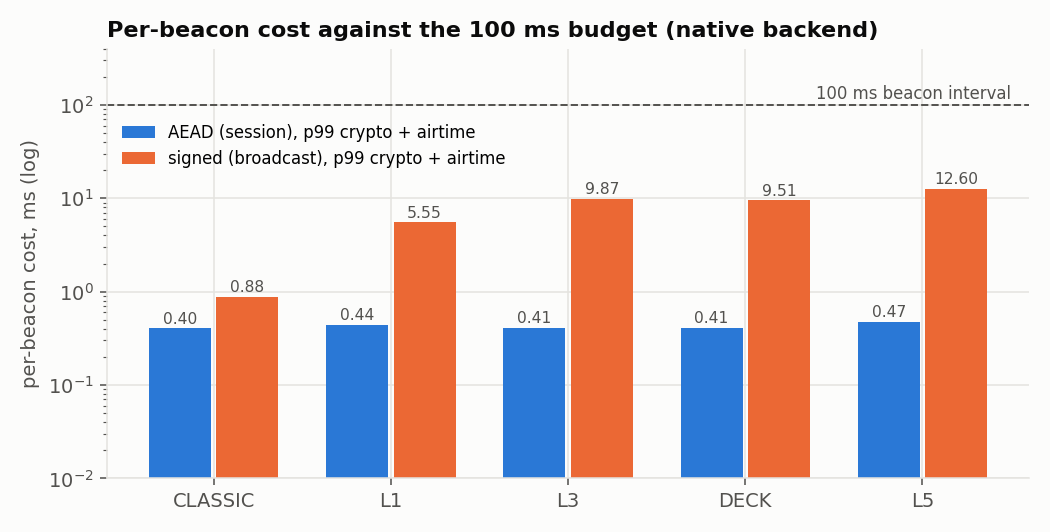
\includegraphics[width=\textwidth]{fig3_beacon_budget.png}
\end{column}
\begin{column}{0.4\textwidth}
\small
\begin{itemize}
\item In a session a beacon is a \V{deck-beacon-aead-bytes}-byte AES-GCM record for \textbf{every} suite: \V{deck-beacon-aead}\,ms of a 100\,ms budget.
\item Signing every beacon fits natively (\V{deck-beacon-signed}\,ms) but costs \V{deck-beacon-signed-frames} frames per beacon.
\item The base paper folds the one-off handshake into per-message latency.
\end{itemize}
\end{column}
\end{columns}
\end{frame}

% -----------------------------------------------------------------------------
\begin{frame}{Result 3: dense traffic breaks post-quantum handshakes}
\centering
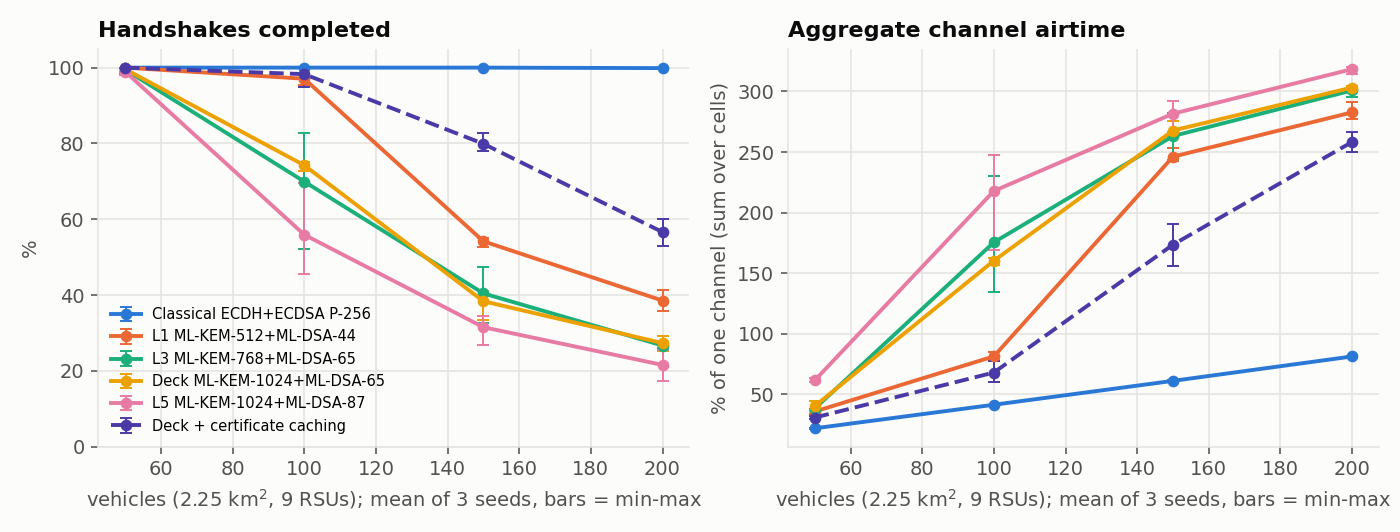
\includegraphics[width=0.92\textwidth]{fig8_ns3_success_airtime.png}

\small Classical: \V{ns3-success-classic-200}\,\% at 200 vehicles. DECK: \V{ns3-success-deck-100}\,\% at 100, \V{ns3-success-deck-200}\,\% at 200. Roughly in order of size (L3 $\approx$ DECK, within seed noise). \textbf{The limit is the channel, not the CPU.}
\end{frame}

% -----------------------------------------------------------------------------
\begin{frame}{Result 4: caching and backoff recover much of it}
\centering
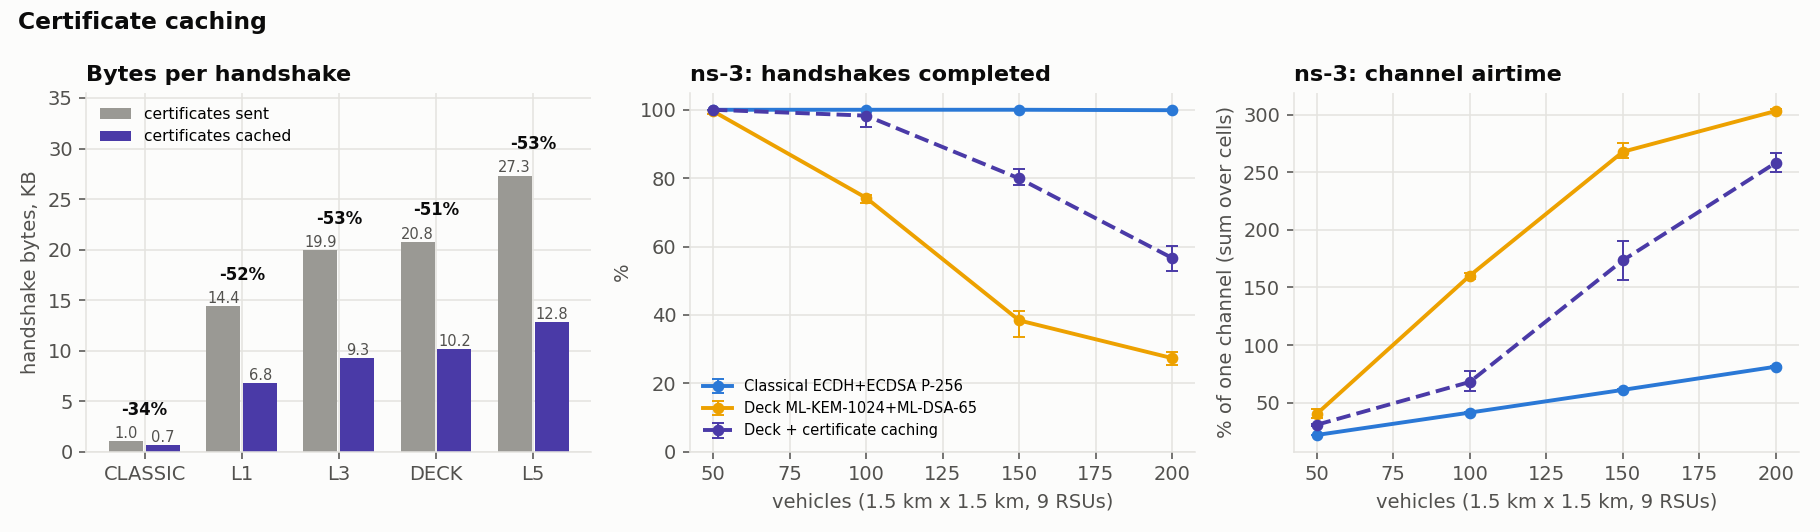
\includegraphics[width=0.95\textwidth]{fig11_cert_cache.png}

\small At 100 vehicles DECK completes \V{ns3-success-deck-100}\,\% $\rightarrow$ \textbf{\V{ns3-success-deck-cache-100}\,\%} with caching; airtime \V{ns3-airtime-deck-100}\,\% $\rightarrow$ \V{ns3-airtime-deck-cache-100}\,\%.\\
Without exponential backoff after failures: \V{var-deck-neither-success}--\V{var-deck-edca-only-success}\,\% complete, alerts wait 380--430\,ms behind handshakes.
\end{frame}

% -----------------------------------------------------------------------------
\begin{frame}{Result 5: AGS-PBFT saves messages, not time}
\begin{columns}[c]
\begin{column}{0.56\textwidth}
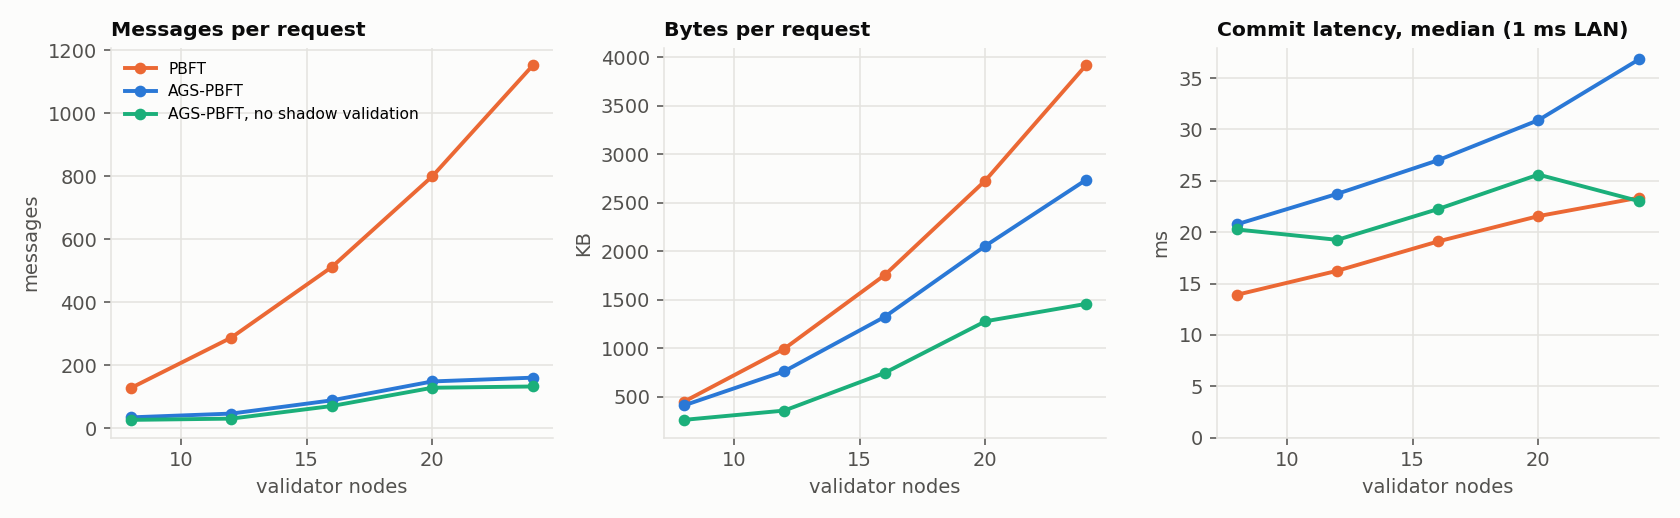
\includegraphics[width=\textwidth]{fig4_consensus_scaling.png}
\end{column}
\begin{column}{0.42\textwidth}
\small
\begin{itemize}
\item \textbf{\V{cons-msg-lo}--\V{cons-msg-hi}\,\% fewer messages}; \V{cons-cpu-lo}--\V{cons-cpu-hi}\,\% less CPU at light load, \V{burst-cpu-more}\,\% \emph{more} under a burst
\item Bytes only \V{cons-byte-lo}--\V{cons-byte-hi}\,\% fewer: blocks carry $2f+1$ ML-DSA signatures
\item Latency \textbf{+\V{cons-lat-lo}--\V{cons-lat-hi}\,\%}: one more hop through the leader
\item Beyond $f$ Byzantine nodes progress stops (leader kept honest in these runs)
\item Weakness: one outlier inflates $\sigma$ and shields a silent node
\end{itemize}
\end{column}
\end{columns}
\end{frame}

% -----------------------------------------------------------------------------
\begin{frame}{Result 6: security}
\small
\textbf{\V{attacks-rejected} of \V{attacks-total} attacks rejected}, each run against the real code:
\begin{columns}[T]
\begin{column}{0.48\textwidth}
\begin{itemize}
\item record tampering, replay, GCM nonce reuse
\item ClientHello replay, stale timestamp
\item client / RSU impersonation with a copied certificate
\item rogue TA, revoked credential, vehicle posing as RSU
\end{itemize}
\end{column}
\begin{column}{0.48\textwidth}
\begin{itemize}
\item MITM on the KEM key or ciphertext, downgrade, tampered Finished
\item forward secrecy
\item claiming another vehicle's cached certificate; revoked but cached
\item forged / spoofed votes, tampered block, rewritten ledger
\end{itemize}
\end{column}
\end{columns}
\vspace{6pt}
Client impersonation \alert{succeeds against the Review 1 design} (no client signature).
\end{frame}

% -----------------------------------------------------------------------------
\begin{frame}{Distributed run (live demo)}
\small
\begin{tabular}{@{}ll@{}}
\toprule
Secure sessions & \V{net-handshakes}; \V{net-rejected} rejected (revoked vehicle) \\
Critical event $\rightarrow$ alert at vehicles & median \V{net-alert-ms}\,ms \\
Event $\rightarrow$ on the ledger & median \V{net-ledger-ms}\,ms \\
Byzantine NODE\_03 & demoted at the first regroup; candidate promoted \\
Leader crash & view change, later events commit \\
Revocation & session closed, reconnection rejected \\
8 ledgers & consistent, verified from genesis (crashed leader's is a prefix) \\
\bottomrule
\end{tabular}

\vspace{8pt}
\code{python scripts/run\_network.py} \quad then the replay viewer: \code{results/viewer.html}
\end{frame}

% -----------------------------------------------------------------------------
\begin{frame}{Findings}
\begin{enumerate}
\item \textbf{Per message, post-quantum V2X fits} the 100\,ms budget at every security level, natively.
\item \textbf{Bandwidth is the binding constraint}: a PQ handshake is $\sim$20$\times$ classical, and dense cells saturate.
\item \textbf{Certificate caching halves the handshake}; exponential backoff prevents congestion collapse.
\item \textbf{DECK = category 3}: L3 gives the same security with a smaller KEM.
\item \textbf{AGS-PBFT}: far fewer messages; slower; never on the safety path.
\end{enumerate}
\end{frame}

% -----------------------------------------------------------------------------
\begin{frame}{Limitations and next steps}
\begin{columns}[T]
\begin{column}{0.48\textwidth}
\textbf{Limitations}
\small
\begin{itemize}
\item Distributed system on one machine; radio only in ns-3
\item ns-3 replays measured costs
\item No WAVE module (ad-hoc MAC)
\item Certificates linkable; no pseudonyms
\item No formal verification
\end{itemize}
\end{column}
\begin{column}{0.48\textwidth}
\textbf{Next}
\small
\begin{itemize}
\item KEM-based authentication (KEMTLS-style) to shrink the handshake further
\item Median/MAD regrouping for AGS-PBFT
\item ProVerif / Tamarin model of the handshake
\item Final report
\end{itemize}
\end{column}
\end{columns}
\end{frame}

\begin{frame}[standout]
Thank you\\[6pt]
\normalsize Questions
\end{frame}

\end{document}
